\clearpage
\noindent This chapter details about the work done till now and the results obtained.
\section{Activities Completed}
\begin{enumerate}
    \item Filtered recent research papers on image description generation using various architecture. From the literature review, found out the literature gaps in recent researches and generated the problem statement.
    \item Completed the image description generation task using Flicker8k dataset with various pre-trained encoders: VGG16, Inception V3 and ResNet50 combined with RNN decoders: LSTM and GRU with and without attention.
    \item Calculated the BLEU-1, BLEU-2, METEOR, GLEU score for all the above mentioned encoder-decoder architecture.
    \item Selected GRU as the decoder based on the time required to train the model.
    \item Deployed all the models and automated the process of selecting the encoders based on the labels obtained from the object detection algorithm.
    \item Built the native mobile application that takes the input as image and predict the description. Converted the generated text description to audio using the Google Text-To-Speech
API.
\end{enumerate}

\section{Results}
\subsection{Encoder-Decoder Image Description Model}
\noindent In our study we adopted encoder-decoder based architecture for generating the image description. We performed an experimental analysis by combining various pre-trained CNN models (encoders) : VGG16, Inception V3, ResNet50, with various sequence generating models (decoders): LSTM and GRU with and without attention mechanism. \\ \\
\noindent The Table \ref{table:2} gives detail of the BLEU-1, BLEU-2 score and Table \ref{table:3} gives detail of the METEOR and GLEU score of above mentioned architectures without attention while training on the Flickr8k dataset. The Table \ref{table:4} gives detail about the time required for training with various model for 20 epochs and 32 batches without attention. \\

\begin{table}[h!]
    \centering
    \caption{BLEU Score for image description model with various encoder and decoder without attention on Flickr8k dataset.}
    \begin{tabular}{ |c|c|c|c|c|c| } 
     \hline
     \textbf{S.No.} & \textbf{Encoder} & \textbf{Decoder} & \textbf{Attention} & \textbf{BLEU-1 Score} & \textbf{BLEU-2 Score}\\ 
     \hline
     1 & VGG16 & LSTM & No & 0.536422 & 0.307395 \\ 
     \hline
     2 & Inception V3 & LSTM & No & \textbf{0.565980}	&  \textbf{0.337752} \\
     \hline
     3 & ResNet50 & LSTM & No & 0.558754 & 0.334540 \\
     \hline
     4 & VGG16 & GRU & No & 0.542930 & 0.313084 \\
     \hline
     5 & Inception V3 & GRU & No & 0.555470 & 0.332273 \\
     \hline
     6 & ResNet50 & GRU & No & 0.551240 & 0.321962 \\
     \hline
    \end{tabular}
    \label{table:2}
\end{table}

\noindent In the Table \ref{table:2}, Inception V3 + LSTM neural network architecture gives the best BLEU-1 and BLEU-2 score, but Inception V3 + GRU neural network architecture gives comparable result. \\

\begin{table}[h!]
    \centering
    \caption{METEOR and GLEU Score for image description model with various encoder and decoder without attention on Flickr8k dataset.}
    \begin{tabular}{ |c|c|c|c|c|c| } 
     \hline
     \textbf{S.No.} & \textbf{Encoder} & \textbf{Decoder} & \textbf{Attention} & \textbf{METEOR Score} & \textbf{GLEU Score}\\ 
     \hline
     1 & VGG16 & LSTM & No & 0.385067 & 0.160952	 \\ 
     \hline
     2 & Inception V3 & LSTM & No & \textbf{0.400490} & \textbf{0.173167} \\
     \hline
     3 & ResNet50 & LSTM & No & 0.398279 & 0.171752 \\
     \hline
     4 & VGG16 & GRU & No & 0.374429 & 0.162264	 \\
     \hline
     5 & Inception V3 & GRU & No & 0.395749 & 0.169225	\\
     \hline
     6 & ResNet50 & GRU & No & 0.386446 & 0.165116 \\
     \hline
    \end{tabular}
    \label{table:3}
\end{table}
\noindent In the Table \ref{table:3},  Inception V3 + LSTM neural network architecture gives the best METEOR and GLEU score, but Inception V3 + GRU neural network architecture gives comparable result.

\begin{table}[h!]
    \centering
    \caption{Training time in min(s) for image description model with various encoder and decoder without attention on Flickr8k dataset.}
    \begin{tabular}{ |c|c|c|c| } 
     \hline
     \textbf{S.No.} & \textbf{Encoder} & \textbf{Decoder} & \textbf{Training Time (min(s))}\\ 
     \hline
     1 & VGG16 & LSTM & 94	 \\ 
     \hline
     2 & Inception V3 & LSTM & 92 \\
     \hline
     3 & ResNet50 & LSTM & 92 \\
     \hline
     4 & VGG16 & GRU & 86	 \\
     \hline
     5 & Inception V3 & GRU & \textbf{84}	\\
     \hline
     6 & ResNet50 & GRU & 91 \\
     \hline
    \end{tabular}
    \label{table:4}
\end{table}
\newpage
\noindent In the Table \ref{table:4}, Inception V3 + GRU neural network architecture gives the least training time because GRU more is less complex than LSTM. In, Table \ref{table:2} & Table \ref{table:3} GRU decoder gave comparable results to LSTM and training time is also less. Hence, we would be considering GRU as our decoder for further study. 

\begin{figure*}[ht!]
    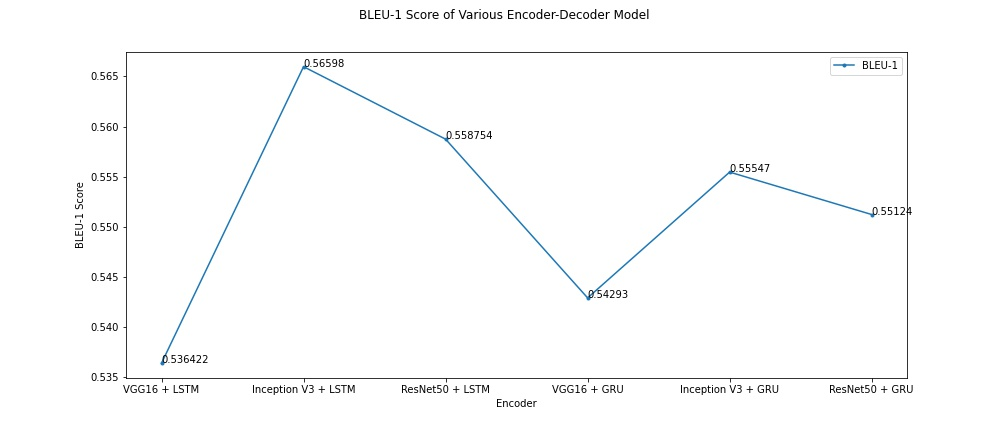
\includegraphics[scale=0.5]{chapters/5/intfig/bleu_score.jpg}\hfill
    \caption{Graphical comparision of BLEU score of different encoder-decoder models without attention on Flickr8k dataset.}
    \label{img:graph_bleu}
\end{figure*}
\noindent In the Figure \ref{img:graph_bleu}, Inception V3 + LSTM neural network architecture gives the best BLEU score, but Inception V3 + GRU neural network architecture gives comparable result.

\begin{figure*}[ht!]
    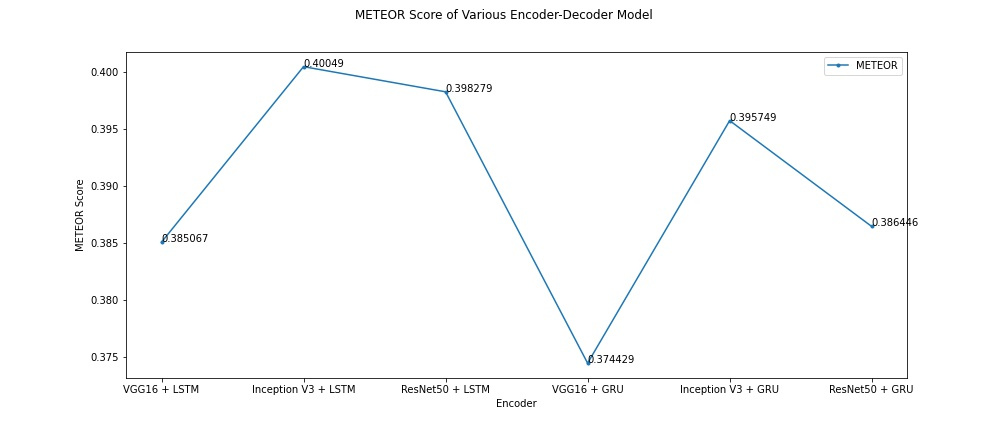
\includegraphics[scale=0.5]{chapters/5/intfig/meteor_score.jpg}\hfill
    \caption{Graphical comparision of METEOR score of different encoder-decoder models without attention on Flickr8k dataset.}
    \label{img:graph_meteor}
\end{figure*}
\newpage
\noindent In the Figure \ref{img:graph_meteor}, Inception V3 + LSTM neural network architecture gives the best METEOR score, but Inception V3 + GRU neural network architecture gives comparable result.

\begin{figure*}[ht!]
    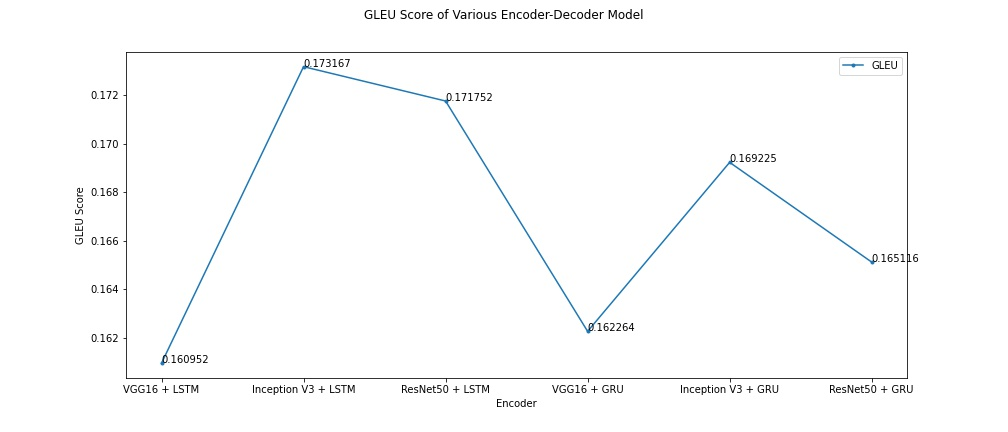
\includegraphics[scale=0.5]{chapters/5/intfig/gleu_score.jpg}\hfill
    \caption{Graphical comparision of GLEU score of different encoder-decoder models without attention on Flickr8k dataset.}
    \label{img:graph_gleu}
\end{figure*}
\noindent In the Figure \ref{img:graph_gleu}, Inception V3 + LSTM neural network architecture gives the best GLEU score, but Inception V3 + GRU neural network architecture gives comparable result.

\begin{figure*}[ht!]
    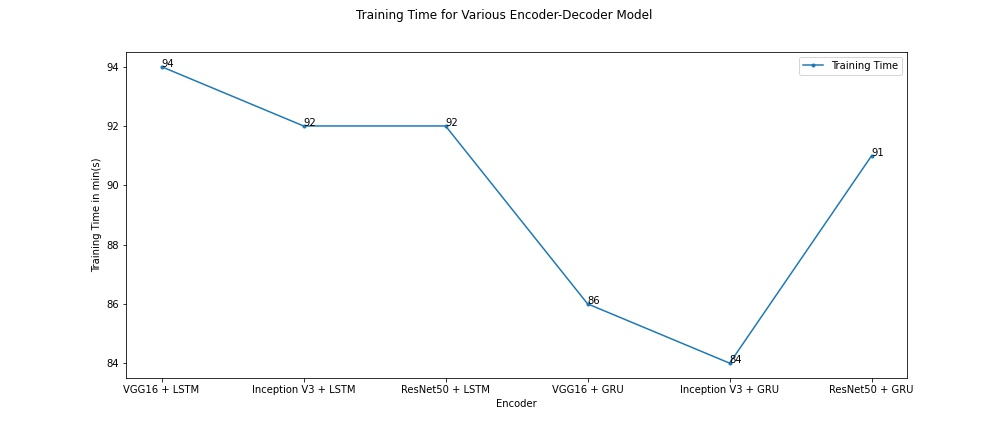
\includegraphics[scale=0.5]{chapters/5/intfig/training_time.jpg}\hfill
    \caption{Graphical comparision for training time of different encoder-decoder models without attention on Flickr8k dataset.}
    \label{img:graph_tt}
\end{figure*}
\noindent Figure \ref{img:graph_tt} shows, Inception V3 + GRU neural network architecture gives the least training time because GRU more is less complex than LSTM. \\ \\ 
\noindent The above graph Figure \ref{img:graph_bleu}, Figure \ref{img:graph_meteor} and Figure \ref{img:graph_gleu}, demonstrates that Inception V3 + LSTM performs best when tested for Flicker8k dataset on various evaluation metrics like BLEU, METEOR and GLEU score. But, Inception V3 + GRU model takes lesser time to train on the same hardware resources and dataset. The BLEU, METEOR and GLEU score also is comparable with the results of the best model. So, we will be considering \textbf{GRU} as our decoder model for further study of image description generation. \\ \\
\noindent The Table \ref{table:5} gives detail of the BLEU-1, BLEU-2 score and Table \ref{table:6} gives detail of the METEOR and GLEU score of various encoders with GRU decoder with attention while training on the Flickr8k dataset. The Table \ref{table:7} gives detail about the time required for training with various model for 20 epochs and 32 batches with attention.

\begin{table}[h!]
    \centering
    \caption{BLEU Score for image description model with various encoder and decoder with attention on Flickr8k dataset.}
    \begin{tabular}{ |c|c|c|c|c|c| } 
     \hline
     \textbf{S.No.} & \textbf{Encoder} & \textbf{Decoder} & \textbf{Attention} & \textbf{BLEU-1 Score} & \textbf{BLEU-2 Score}\\ 
     \hline
     1 & VGG16 & GRU & Yes & 0.544142 & 0.332934 \\
     \hline
     2 & Inception V3 & GRU & Yes & 0.586869 & \textbf{0.338021} \\
     \hline
     3 & ResNet50 & GRU & Yes & \textbf{0.596845} & 0.337755 \\
     \hline
    \end{tabular}
    \label{table:5}
\end{table}
\newpage
\noindent In the Table \ref{table:5}, Resnet50 gives the best BLEU-1 score, while Inception V3 gives the best BLEU-2 score. The table demonstrates the uncertainty between the encoders.

\begin{table}[h!]
    \centering
    \caption{METEOR and GLEU Score for image description model with various encoder and decoder with attention on Flickr8k dataset.}
    \begin{tabular}{ |c|c|c|c|c|c| } 
     \hline
     \textbf{S.No.} & \textbf{Encoder} & \textbf{Decoder} & \textbf{Attention} & \textbf{METEOR Score} & \textbf{GLEU Score}\\ 
     \hline
     4 & VGG16 & GRU & Yes & 0.454923 & 0.174830	 \\
     \hline
     5 & Inception V3 & GRU & Yes & 0.436624 & 0.172741	\\
     \hline
     6 & ResNet50 & GRU & Yes & \textbf{0.515464} & \textbf{0.206574} \\
     \hline
    \end{tabular}
    
    \label{table:6}
\end{table}
\noindent Table \ref{table:6} shows that Resnet50 gives the best METEOR and GLEU score amongst all the other encoders.

\begin{table}[h!]
    \centering
    \caption{Training time in min(s) for image description model with various encoder and decoder with attention on Flickr8k dataset.}
    \begin{tabular}{ |c|c|c|c| } 
     \hline
     \textbf{S.No.} & \textbf{Encoder} & \textbf{Decoder} & \textbf{Training Time (min(s))}\\ 
     \hline
     4 & VGG16 & GRU & \textbf{240}	 \\
     \hline
     5 & Inception V3 & GRU & 275	\\
     \hline
     6 & ResNet50 & GRU & 280 \\
     \hline
    \end{tabular}
    \label{table:7}
\end{table}

 \noindent GRU gave the best training time as showed in Table \ref{table:4}. But, amongst the various encoder VGG16 in the Table \ref{table:7} took the least time to train the model, because of the less number of layers to train in VGG16 encoder model. But, we cannot compromise with the accuracy of the image description generation. Hence, to resolve the uncertainity between different encoders, we will automate the selection of encoders.
 
\newpage
\begin{figure*}[ht!]
    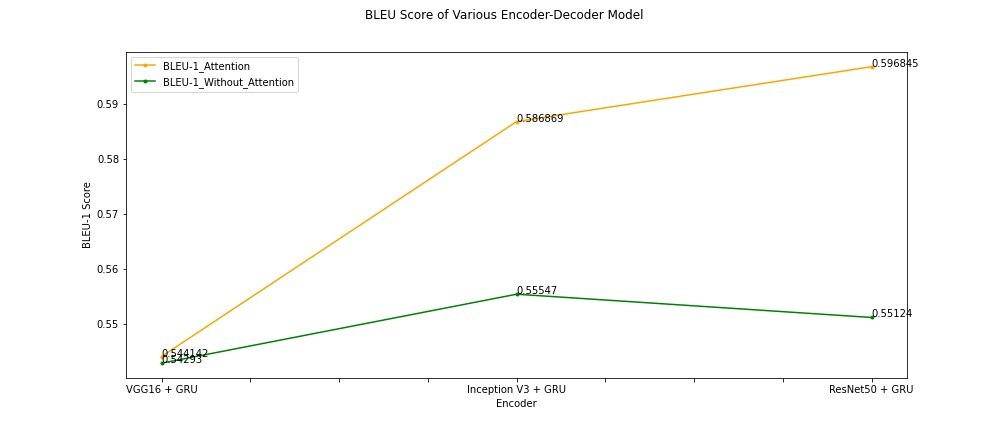
\includegraphics[scale=0.5]{chapters/5/intfig/bleu-1_score_attention.jpg}\hfill
    \caption{Graphical comparision of BLEU-1 score of different encoder-decoder models with and without attention on Flickr8k dataset.}
    \label{img:graph_bleu-1_attention}
\end{figure*}

\noindent The graphical plot \ref{img:graph_bleu-1_attention} demonstrates there is increase in the BLEU-1 score of various encoder-decoder based model using the attention mechanism.

\begin{figure*}[ht!]
    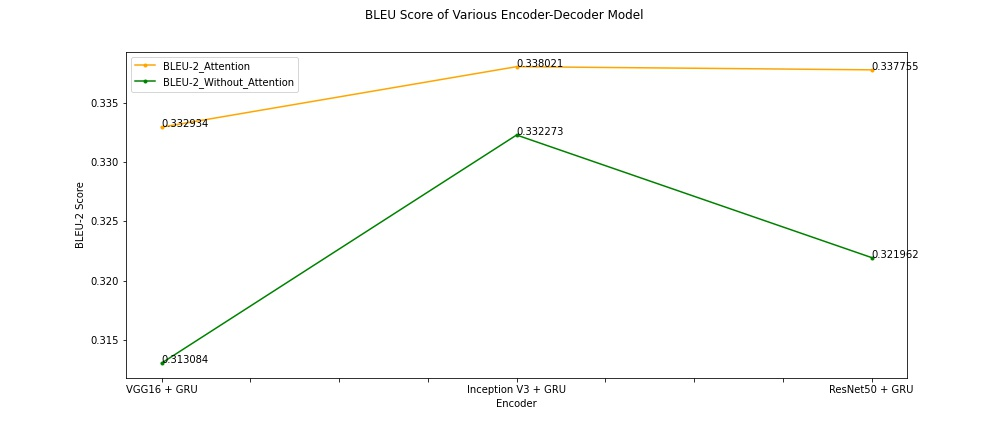
\includegraphics[scale=0.5]{chapters/5/intfig/bleu-2_score_attention.jpg}\hfill
    \caption{Graphical comparision of BLEU-2 score of different encoder-decoder models with and without attention on Flickr8k dataset.}
    \label{img:graph_bleu-2_attention}
\end{figure*}

\noindent The graphical plot \ref{img:graph_bleu-2_attention} demonstrates there is increase in the BLEU-2 score of various encoder-decoder based model using the attention mechanism.

\begin{figure*}[ht!]
    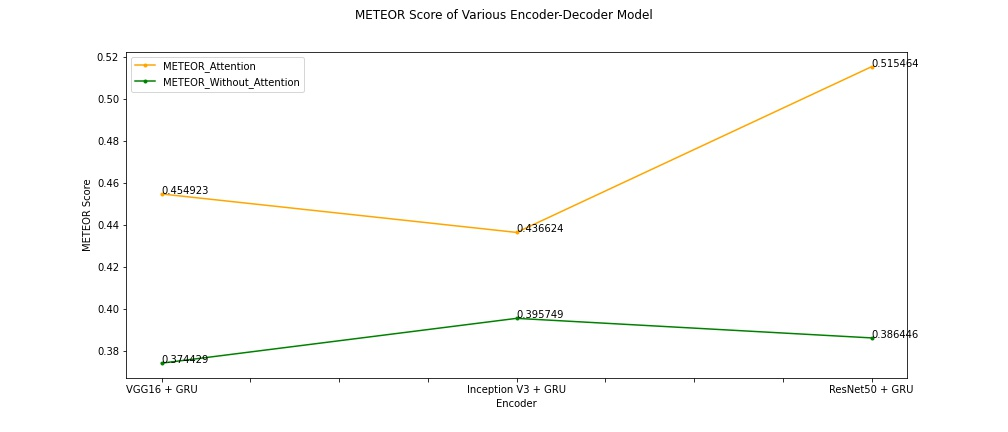
\includegraphics[scale=0.5]{chapters/5/intfig/meteor_score_attention.jpg}\hfill
    \caption{Graphical comparision of METEOR score of different encoder-decoder models with and without attention on Flickr8k dataset.}
    \label{img:meteor_attention}
\end{figure*}

\noindent The graphical plot \ref{img:meteor_attention} demonstrates there is increase in the METEOR score of various encoder-decoder based model using the attention mechanism.

\begin{figure*}[ht!]
    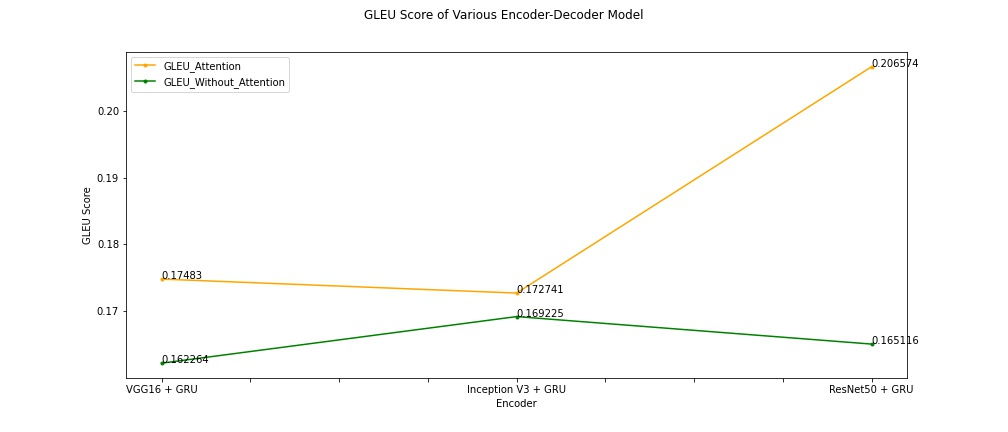
\includegraphics[scale=0.5]{chapters/5/intfig/gleu_score_attention.jpg}\hfill
    \caption{Graphical comparision of GLEU score of different encoder-decoder models with and without attention on Flickr8k dataset.}
    \label{img:gleu_attention}
\end{figure*}

\noindent The graphical plot \ref{img:gleu_attention} demonstrates there is increase in the GLEU score of various encoder-decoder based model using the attention mechanism.

\newpage
\noindent
The above results demonstrates that attention mechanism definitely increased scores of all evaluation metrics: BLEU-1, BLEU-2, METEOR and GLEU. However, there is uncertainty around the selection of encoder. So, we would be deploying all the models with encoder as VGG-16, InceptionV3 and ResNet50. We would automate the process of selection of encoders based on the matching labels achieved from the object detection algorithm.\\ 
\noindent Here, are some screenshots of the generated image descriptions from various encoders with attention.

\begin{figure*}[ht!]
    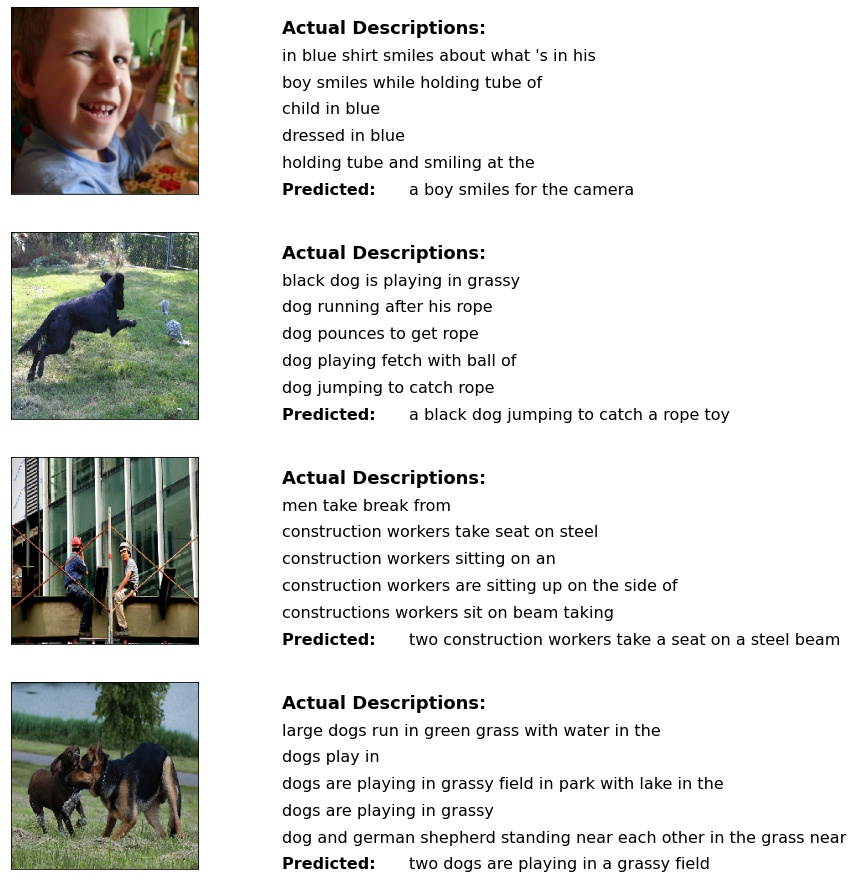
\includegraphics[scale=0.4]{chapters/5/intfig/vgg16_and_gru_with_attention_output.jpg}
    \caption{Sample description of images generated using VGG16 as encoder and GRU as decoder with attention.}
    \label{res:vgg16_gru_attention}
\end{figure*}

\noindent In the Figure \ref{res:vgg16_gru_attention}, the predicted captions are able to identify the object, action and attributes present in the image. The attention mechanism certainly helps in improving the generate captions. When using VGG16 as encoder, generated features are less as compared to InceptionV3 and ResNet50 because of less number of layers to train. \\ \\

\begin{figure*}[ht!]
    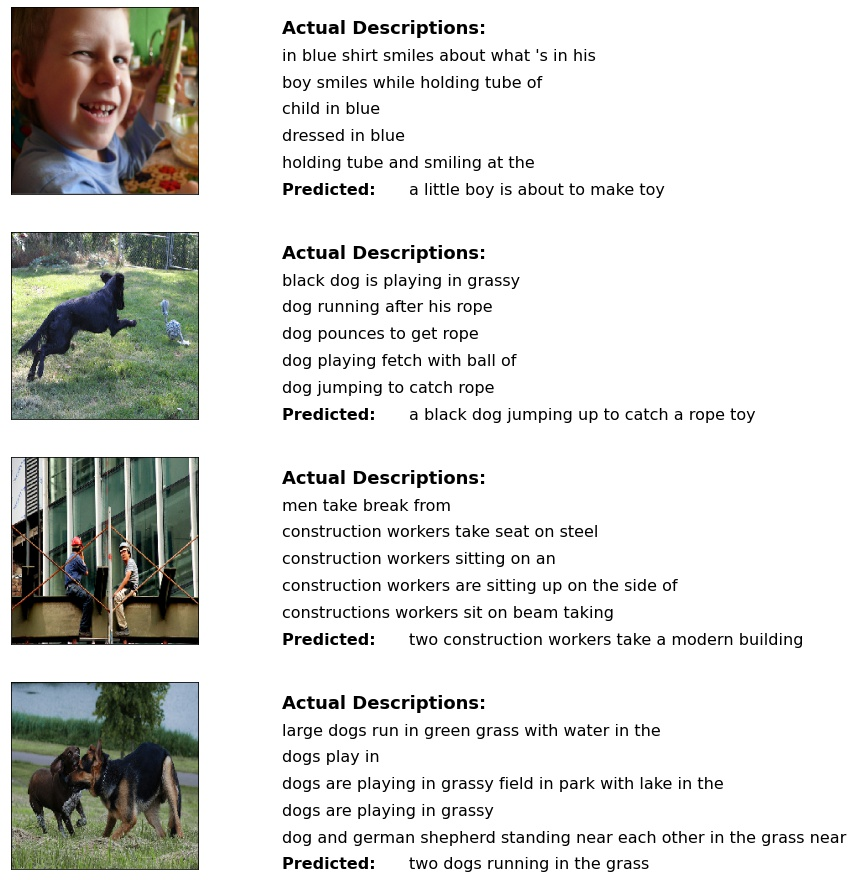
\includegraphics[scale=0.4]{chapters/5/intfig/inception_and_gru_with_attention_output.jpg}
    \caption{Sample description of images generated using Inception V3 as encoder and GRU as decoder with attention.}
    \label{res:inceptionv3_gru_attention}
\end{figure*}

\noindent In the Figure \ref{res:inceptionv3_gru_attention}, the features identified in the images are more as compared to \ref{res:vgg16_gru_attention} because of more number of training layers. But, there are some abnormalities find in the generated in the above architecture as well. This will be solved by automating the selection of encoders.
\newpage
\begin{figure*}[ht!]
    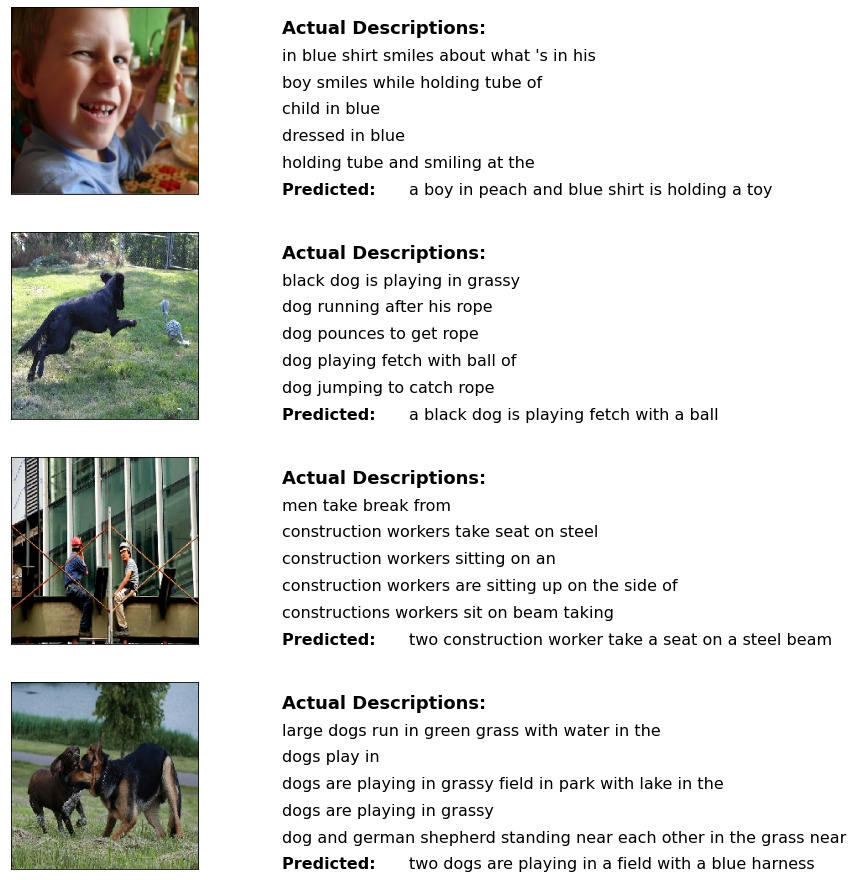
\includegraphics[scale=0.35]{chapters/5/intfig/resnet_and_gru_with_attention_output.jpg}
    \caption{Sample description of images generated using ResNet50 as encoder and GRU as decoder with attention.}
    \label{res:resnet50_gru_attention}
\end{figure*}
\noindent In the Figure \ref{res:resnet50_gru_attention}, the features identified in the images are more as compared to \ref{res:vgg16_gru_attention} and \ref{res:inceptionv3_gru_attention} because of more number of training layers.

\begin{figure*}[ht!]
    \begin{center}
        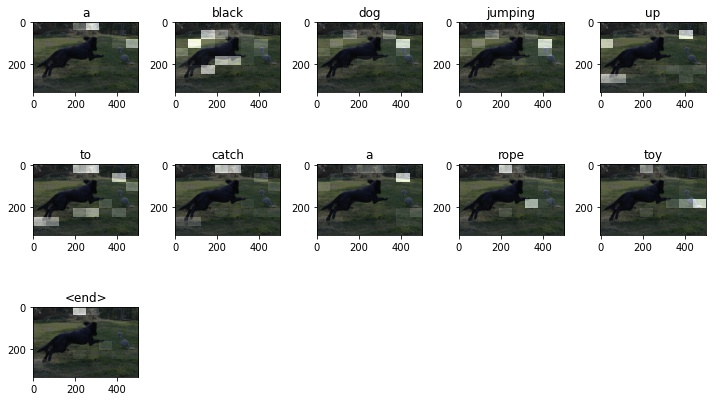
\includegraphics[scale=0.45]{chapters/5/intfig/inception_and_gru_with_attention_plot_attention.jpg}
    \end{center}
    \caption{Sample attention plot for the image description generation}
    \label{res:attention_plot2}
\end{figure*}

\begin{figure*}[ht!]
    \begin{center}
        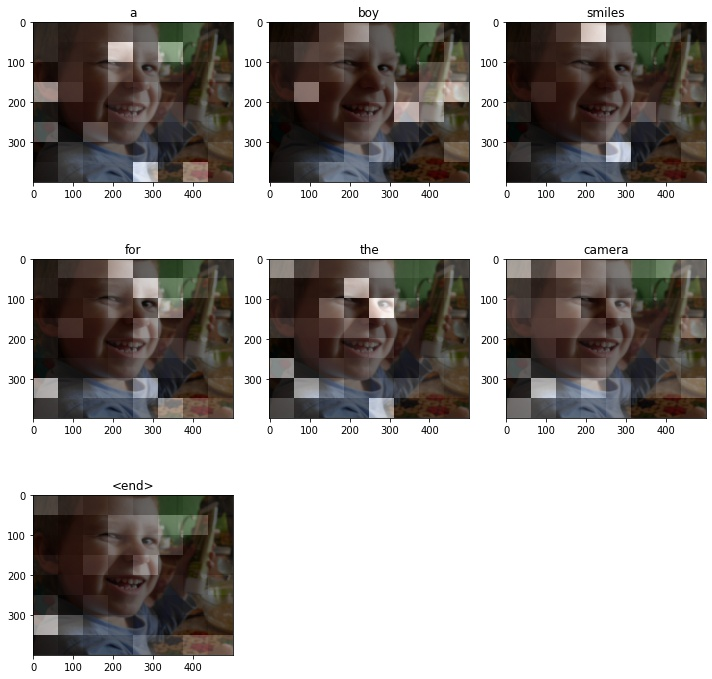
\includegraphics[scale=0.5]{chapters/5/intfig/vgg16_and_gru_with_attention_plot_attention.jpg}
    \end{center}
    \caption{Sample attention plot for the image description generation}
    \label{res:attention_plot}
\end{figure*}

\noindent In the Figure \ref{res:attention_plot2} and \ref{res:attention_plot}, gives the plot of the attention map for each word predicted. The word instead of using the entire image, focuses on certain region of the map which represent that word more accurately.

\noindent To deal with the uncertainty between different encoders and improving the accuracy of the image description, we automated the process
of selection of encoders. For each image, the encoder with
the maximum matching root words with the labels obtained
from label detection algorithm will be considered best. After
experimenting with the automated neural network architecture,
we achieved a BLEU-1 score of \textbf{0.619}. We achieved our goal
of reducing the training time by using GRU decoder and
improving the accuracy by automating the process of selection
of encoders.
